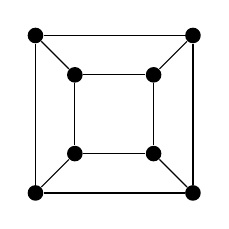
\begin{tikzpicture}[scale=1]
\tikzset{knoten/.style={circle,fill=black,inner sep=0.7mm}}
\node [knoten] (a) at (0,0) {};
\node [knoten] (b) at (2,0) {};
\node [knoten] (c) at (2,2) {};
\node [knoten] (d) at (0,2) {};
\node [knoten] (e) at (0.5,0.5) {};
\node [knoten] (f) at (1.5,0.5) {};
\node [knoten] (g) at (1.5,1.5) {};
\node [knoten] (h) at (0.5,1.5) {};
\draw[-] (a) to (b);
\draw[-] (b) to (c);
\draw[-] (c) to (d);
\draw[-] (d) to (a);
\draw[-] (e) to (f);
\draw[-] (f) to (g);
\draw[-] (g) to (h);
\draw[-] (h) to (e);
\draw[-] (a) to (e);
\draw[-] (b) to (f);
\draw[-] (c) to (g);
\draw[-] (d) to (h);
\end{tikzpicture}
